\chapter{SO SÁNH TỔNG HỢP, XU HƯỚNG VÀ KHUYẾN NGHỊ}

\section{Bảng tổng quan tất cả phiên bản}

\begin{table}[H]\centering
\caption{Tổng quan các phiên bản YOLO (2015--2026)}
\scriptsize
\begin{tabular}{lcccccccc}\toprule
\textbf{Version} & \textbf{Năm} & \textbf{mAP VOC@50} & \textbf{mAP COCO@50:95} & \textbf{FPS (GPU)} & \textbf{Params} & \textbf{Anchor} & \textbf{NMS} & \textbf{Paper}\\\midrule
v1 \cite{yolov1} & 2015 & 63.4\% & --- & 45 (Titan X) & $\sim$45M & Grid & Cần & Có \\
v2 \cite{yolov2} & 2016 & 78.6\% & --- & 67 (Titan X) & $\sim$50M & Có & Cần & Có \\
v3 \cite{yolov3} & 2018 & --- & 33.0\% & 20 (Titan X) & $\sim$62M & Có & Cần & Có \\
v4 \cite{yolov4} & 2020 & --- & 43.5\% & 65 (V100) & $\sim$64M & Có & Cần & Có \\
v5 \cite{yolov5} & 2020 & --- & 50.7\% & 98 (V100) & 86.7M & Có & Cần & Không \\
v6 \cite{yolov6} & 2022 & --- & 52.5\% & 116 (T4) & $\sim$58M & Không & Cần & Có \\
v7 \cite{yolov7} & 2022 & --- & 56.8\% & 36 (V100) & $\sim$71M & Có & Cần & Có \\
v8 \cite{yolov8} & 2023 & --- & 53.9\% & 83 (T4) & 68.2M & Không & Cần & Không \\
v9 \cite{yolov9} & 2024 & --- & 55.6\% & 57 (T4) & 58.1M & Không & Cần & Có \\
v10 \cite{yolov10} & 2024 & --- & 54.4\% & 96 (T4) & 29.5M & Không & \textbf{Không} & Có \\
YOLO11 \cite{yolo11} & 2024 & --- & 54.7\% & 79 (T4) & 56.9M & Không & \textbf{Cần} & Không \\
v12 \cite{yolov12} & 2025 & --- & 55.2\% & 51 (T4) & 59.1M & Không & Không & Có \\
YOLO26 \cite{yolo26} & 2026 & --- & $\sim$57.2\% & $\sim$102 (T4)$^*$ & $\sim$60M & Không & Không & Không \\
\bottomrule
\end{tabular}
\end{table}

\textit{$^*$ Ước tính. FPS = model size lớn nhất (v7-E6E, v5x, v8x...) trừ v1--v3 (model duy nhất). GPU ghi trong ngoặc. Lưu ý: Titan X, V100, T4 là 3 thế hệ GPU khác nhau --- FPS giữa chúng \textbf{không so sánh trực tiếp được}. v1--v2 dùng mAP VOC@50, v3+ dùng mAP COCO@50:95 --- hai thang đo hoàn toàn khác nhau.}

\section{Tiến hóa kiến trúc}

\begin{table}[H]\centering
\caption{Tiến hóa các thành phần qua 11 năm}
\begin{tabular}{ll}\toprule
\textbf{Thành phần} & \textbf{Tiến hóa}\\\midrule
\textbf{Backbone} & CNN 24-layer $\rightarrow$ Darknet-53 $\rightarrow$ CSPDarknet $\rightarrow$ E-ELAN $\rightarrow$ Area Attention \\
\textbf{Anchor} & Grid (v1) $\rightarrow$ Anchor-based (v2--v7) $\rightarrow$ Anchor-free (v6,v8+) \\
\textbf{NMS} & Cần NMS (v1--v9) $\rightarrow$ NMS-free Dual Assignment (v10+) \\
\textbf{Loss} & MSE $\rightarrow$ IoU $\rightarrow$ CIoU + DFL (v8) $\rightarrow$ Bỏ DFL (YOLO26) \\
\textbf{Framework} & Darknet C (v1--v4) $\rightarrow$ PyTorch pip install (v5+) \\
\bottomrule
\end{tabular}
\end{table}

\section{Biểu đồ Pareto: Params vs mAP}

\begin{figure}[H]
\centering
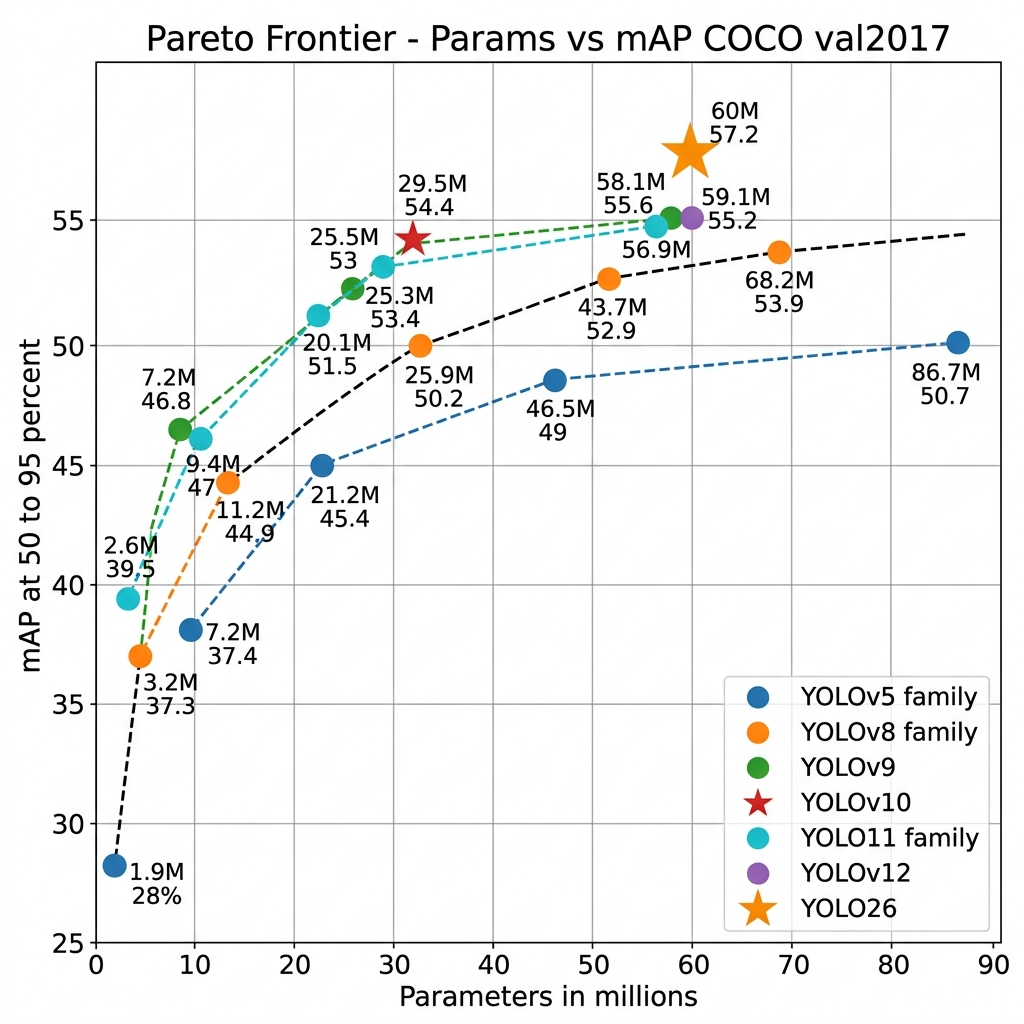
\includegraphics[width=0.9\textwidth]{pareto_chart.png}
\caption{Biểu đồ Pareto (Params vs mAP COCO@50:95). Góc \textbf{trên-trái} = hiệu quả nhất (ít params, mAP cao). YOLO26-X và YOLOv10-X nằm trên đường biên Pareto.}
\end{figure}

\section{Trade-off: Version ``thua'' đời trước}

\begin{table}[H]\centering
\caption{Phân tích trade-off}
\begin{tabular}{lll}\toprule
\textbf{Trường hợp} & \textbf{Thua ở đâu} & \textbf{Thắng ở đâu}\\\midrule
v8 thua v7 \cite{yolov7}\cite{yolov8} & mAP: 53.9\% < 56.8\% & Multi-task (6 tác vụ), ecosystem \\
v10 thua v9 \cite{yolov9}\cite{yolov10} & mAP: 54.4\% < 55.6\% & Params 2$\times$ ít hơn, NMS-free \\
v3 chậm hơn v2 \cite{yolov2}\cite{yolov3} & FPS: 20 < 67 & mAP tốt hơn nhiều \\\bottomrule
\end{tabular}
\end{table}

\textbf{Bài học:} Không version nào thua hoàn toàn. Mỗi ``thua'' là \textbf{trade-off có chủ đích}.

\section{Xếp hạng theo tiêu chí}

\subsection{Accuracy thuần túy (mAP COCO@50:95)}
\begin{enumerate}
    \item YOLO26-X: $\sim$57.2\% \cite{yolo26}
    \item YOLOv7-E6E: 56.8\% \cite{yolov7}
    \item YOLOv9-E: 55.6\% \cite{yolov9}
    \item YOLOv12-X: 55.2\% \cite{yolov12}
    \item YOLO11-X: 54.7\% \cite{yolo11}
\end{enumerate}

\subsection{Efficiency (mAP/Params)}
YOLOv10-X dẫn đầu: 54.4\% mAP với chỉ 29.5M params (1.84 mAP/M) \cite{yolov10}.

\subsection{Production readiness (2026)}
YOLO11 > YOLOv8 > YOLO26 > YOLOv12

\section{Sơ đồ phả hệ YOLO (Family Tree)}

\begin{figure}[H]
\centering
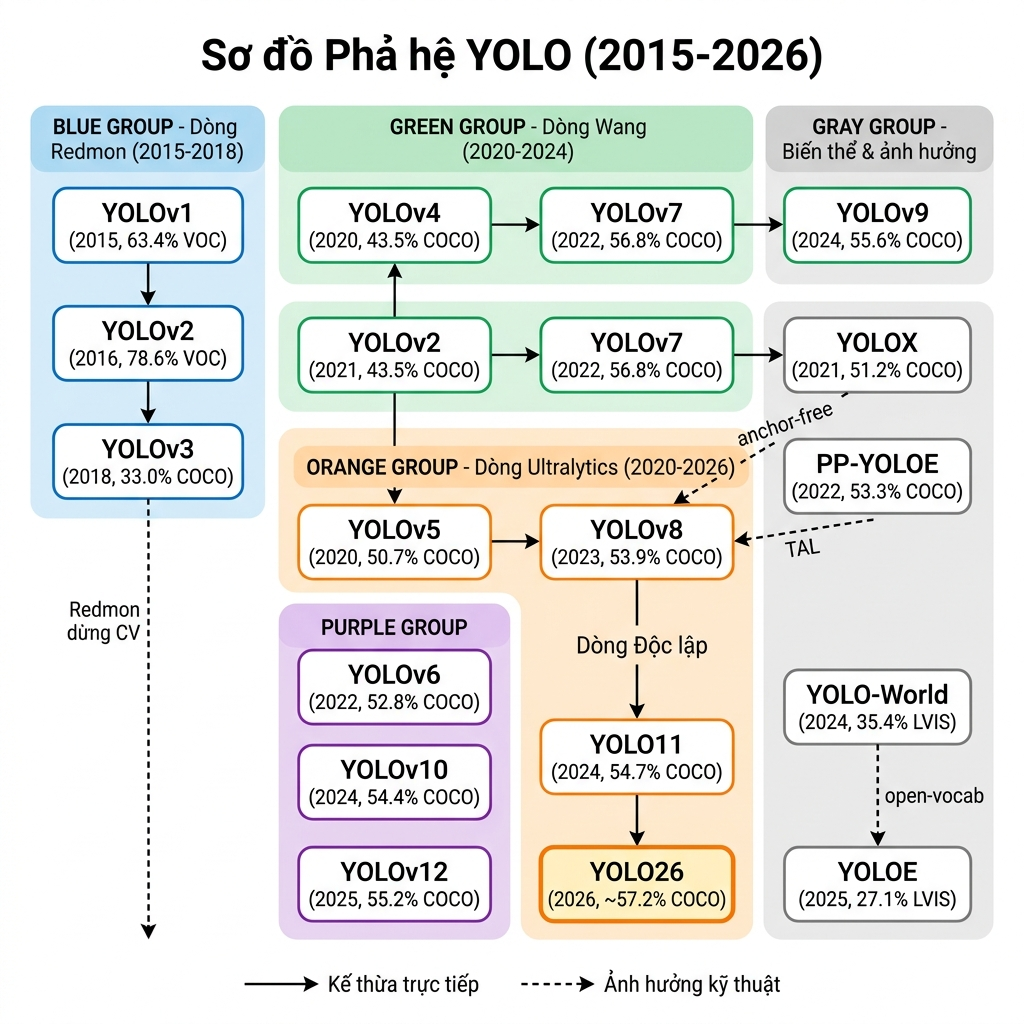
\includegraphics[width=\textwidth]{yolo_family_tree.png}
\caption{Sơ đồ phả hệ các phiên bản YOLO (2015--2026). Đường liền: kế thừa trực tiếp. Đường nét đứt: ảnh hưởng kỹ thuật.}
\end{figure}

\section{Xu hướng phát triển}

\begin{enumerate}
    \item \textbf{CNN $\rightarrow$ Attention:} v12 mở đầu, tương lai hybrid CNN+Attention
    \item \textbf{Closed-set $\rightarrow$ Open-vocabulary:} YOLOE detect vật chưa train \cite{yoloe}
    \item \textbf{Server $\rightarrow$ Edge:} YOLO26 tối ưu NPU, INT8, mobile \cite{yolo26}
    \item \textbf{NMS $\rightarrow$ NMS-free:} End-to-end detection từ v10 \cite{yolov10}
    \item \textbf{CV $\leftarrow$ NLP:} Cross-pollination từ LLM (MuSGD, CLIP)
    \item \textbf{Detection $\rightarrow$ Multi-task:} 1 model cho detect+segment+pose+track \cite{yolov8}
\end{enumerate}

\section{Khuyến nghị chọn model}

\begin{table}[H]\centering
\caption{Hướng dẫn chọn phiên bản YOLO theo mục đích}
\begin{tabular}{lll}\toprule
\textbf{Mục đích} & \textbf{Chọn} & \textbf{Lý do}\\\midrule
Accuracy tối đa & YOLO26-X / v7-E6E & mAP cao nhất \cite{yolov7}\cite{yolo26} \\
Dễ dùng, đa năng & v8 / YOLO11 & pip install, 6 tasks \cite{yolov8} \\
Deploy NPU/edge & YOLO26-N / v10-N & NMS-free, INT8-friendly \cite{yolov10}\cite{yolo26} \\
Ít params nhất & YOLOv10-X & 29.5M cho 54.4\% \cite{yolov10} \\
Real-time cực nhanh & YOLOv6-S & 520+ FPS TensorRT \cite{yolov6} \\
Detect vật chưa train & YOLOE & Open-vocab, 3 modes \cite{yoloe} \\
Vật nhỏ (drone) & YOLO26 & STAL chuyên vật nhỏ \cite{yolo26} \\
INT8 quantization & YOLO-NAS & Mất chỉ 0.4\% \cite{yolonas} \\
Học/nghiên cứu & v1$\rightarrow$v4 papers & Nền tảng lý thuyết \cite{yolov1}\cite{yolov4} \\\bottomrule
\end{tabular}
\end{table}
